\documentclass[]{scrartcl}
\usepackage{graphicx}
\usepackage{subfig}
\usepackage{amsmath}
\usepackage{xcolor}
\usepackage[round,sort]{natbib}
\usepackage{natbib}

%opening
\title{BMT1D.py  Programs for 1D Bayesian inversion of magnetotelluric data considering model discrepancy}
\author{Ho\"{e}l Seill\'{e} \& Gerhard Visser \thanks{CSIRO Deep Earth Imaging FSP, Perth, Australia}}



\begin{document}
	
	\maketitle

	\section{Introduction and overview of the programs}
	
	The present document describes the workflow to perform 1D Bayesian inversions of magnetotelluric (MT) data considering dimensionality discrepancies. The workflow is described using 3 synthetic MT soundings as example. Refer to the paper "Bayesian inversion of magnetotelluric data considering dimensionality discrepancies" \citep{Seille2020a} for more details about the algorithm and the workflow. The synthetic soundings presented in the paper are the ones included in this software for testing. 
	
	The workflow can be divided into three main steps: The MT data is analysed and prepared for the inversion using a suite of Python scripts. The inversion is ran using a C executable. The outputs of the inversion are read and analysed using another suite of Python scripts.
	
	\begin{itemize}
		\item \textbf{DDE}: Dimensionality Discrepancy Estimation: Using input MT data in the form of EDI files and an existing ``Dimensionality Discrepancy model", this program computes the phase tensor parameters in order to estimate the ``site-specific likelihood" functions reflective of uncertainty caused by the presence of 2D and 3D effects. This uncertainty is summed up to the processing noise variance/covariance matrix and stored alongside the data (determinant of the full impedance tensor) into in a \textit{.csv} file for use into the probabilistic algorithm.
		
		\item \textbf{transdMT}: Trans-dimensional Markov chain Monte Carlo probabilistic algorithm. The  \textit{.csv} files created by the DDE.py program is used as the data input file by the program. Parameters of the inversion are specified in a separate file. The output of the inversion are binary files which contains the ensembles of models and responses. 
		
		\item \textbf{plotResultsMCMC}: Read and plot the posterior ensembles. 

	\end{itemize}
		
	
	
	\section{Dependencies}
	
	This section describes the dependencies required by the programs to run.
	The python libraries that are used by the program are:
	
	\begin{itemize}
	\item[--] numpy
	\item[--] pandas
	\item[--] scipy
	\item[--] matplotlib
	\item[--] sys
	\item[--] os
	\item[--] re
	\item[--] numba
	\end{itemize}
	
	The present suite of Python scripts and the executable have been tested on a Linux environment, with Python 3.6 installed. The Python scripts can also be run on Windows.
	
	\section{Directory structure}
	
	\begin{verbatim}
	
	projects/           --> all inputs and outputs files and images
	   example/         --> folder for the project example
	      csv/          --> csv files for the transdMT program
	      edi/          --> EDI files for DDE.py
	      posteriors/   --> files for ensembles.py
	      tree/         --> files defining the DDM
	
	src/                --> all source files and scripts

	
	\end{verbatim}
	
	\section{DDE}
	The \textbf{editMTdata.py} computes the determinant of the full impedance tensor and the uncertainty to consider within the inversion (1D dimensionality plus processing uncertainty).
	Most of the processed MT data is found in the form of EDI files \citep{Wight1987}. It contains data in form of the full complex impedance Tensor Z at each frequency, and the variance associated to each element of the tensor. The variance is real and common to both real and imaginary parts of each element of Z, assuming a circularly-symmetric complex normal distribution. The script that reads the EDI files accepts a standard format, the same as the one used by the WinGLink software when exporting the EDI files.   
	If the full noise covariance matrix is available, it is possible to use it, to take into account correlated errors across frequencies. This implementation has not been tested thoroughly yet. %\citep[e.g.][]{Kelbert2020,Xiang2018}. 

	\bigbreak
	The (edited) EDI files have to be placed in \textit{projects/example/edi/}. The attribute list and the tree file are in \textit{projects/example/tree/}. An optimal DDM (\textit{tree.txt}) is made available \citep[see][]{Seille2020a}. In case an another DDM wants to be specified, refer to section \ref{custom_tree}.
	\bigbreak
	
	Several options related to the DDE preparation step are available to run the script, and are fed as arguments to the script.	The options are:
	
	\begin{verbatim}
		
		EF             --> error floor. If EF > 0, it will use this error floor value 
						and will ignore the DDM.
		medfiltsp      --> if specified, define the log spacing to perform the 
						median filtering. Default value is 0.2. Larger values will 
						result in an increased smoothing of the PT parameters.
		plotMTdata     --> plot the EDI file and Phase tensor parameters.
		saveCSVfiles   --> save the soundings to .csv for the inversion.
		
	\end{verbatim}
	
	\textbf{DDE.py}: Within the \textit{project/example/} folder, run the script with these instructions: 
		
	\begin{verbatim}
	python3 ../../src/DDE.py Error_Floor median_filter 
	           boolean_for_plotMTdata boolean_for_saveCSVfiles
	\end{verbatim}
	
	\bigbreak
	For example, to prepare the input using the DDM and save and plot the data:
	\begin{verbatim}
	python3 ../../src/DDE.py /tree/atts.txt /tree/tree.txt -1 0.2 True True
	\end{verbatim} 
	
	\bigbreak
	For example, to prepare the input using an error floor of 5\% and save and plot the data:
	\begin{verbatim}
	python3 ../../src/DDE.py None None 0.05 0.2 True True
	\end{verbatim} 

    If using an error floor, the resulting csv file will have appended the string 'EF'.
	
		
	\bigbreak
	The input data images are saved in the same folder as the EDI files. It serves at a first QC to ensure that no outliers are present in the Phase tensor (PT) parameters $\beta$ and $\lambda$. Careful edition of the data prior to running the script is sought. Obvious outliers should be removed. Use of the D+ solution \citep{Beamish1992} to infer the presence of noise or physically invalid responses is recommended.
	
	Outliers in the PT parameters might be assimilated by the DDE algorithm as data having a high-order dimensionality. If encountered at high frequencies the rest of the frequency range will also be considered as having a high-order dimensionality. It is why it is crucial to remove outliers or data suspected to be noisy at this stage of the workflow. In the presence of this type of outliers the input data should be reedited and the process of creating the input file repeated. Images created by the script for the EDI present in the example folder are shown in Fig. \ref{EDI2MTUL_figs}.
	
	% TODO
	%\bigbreak
	%\textbf{editMTdata.py}. To remove noisy data an additional script is available. The MT site  and the list of frequencies to be removed has to be specified as an argument when calling the script. Script usage: 
	
	%\begin{verbatim}
	%python3 ../../src/editMTdata.py [edi_file_name] [frequency list]
	%\end{verbatim}
	
	%For example:
	%\begin{verbatim}
	%python3 ../../src/editMTdata.py edi/065.edi [5,6,7,8,9,10]
    %\end{verbatim} 


	\begin{figure}
		\centering
		\subfloat[MT065]{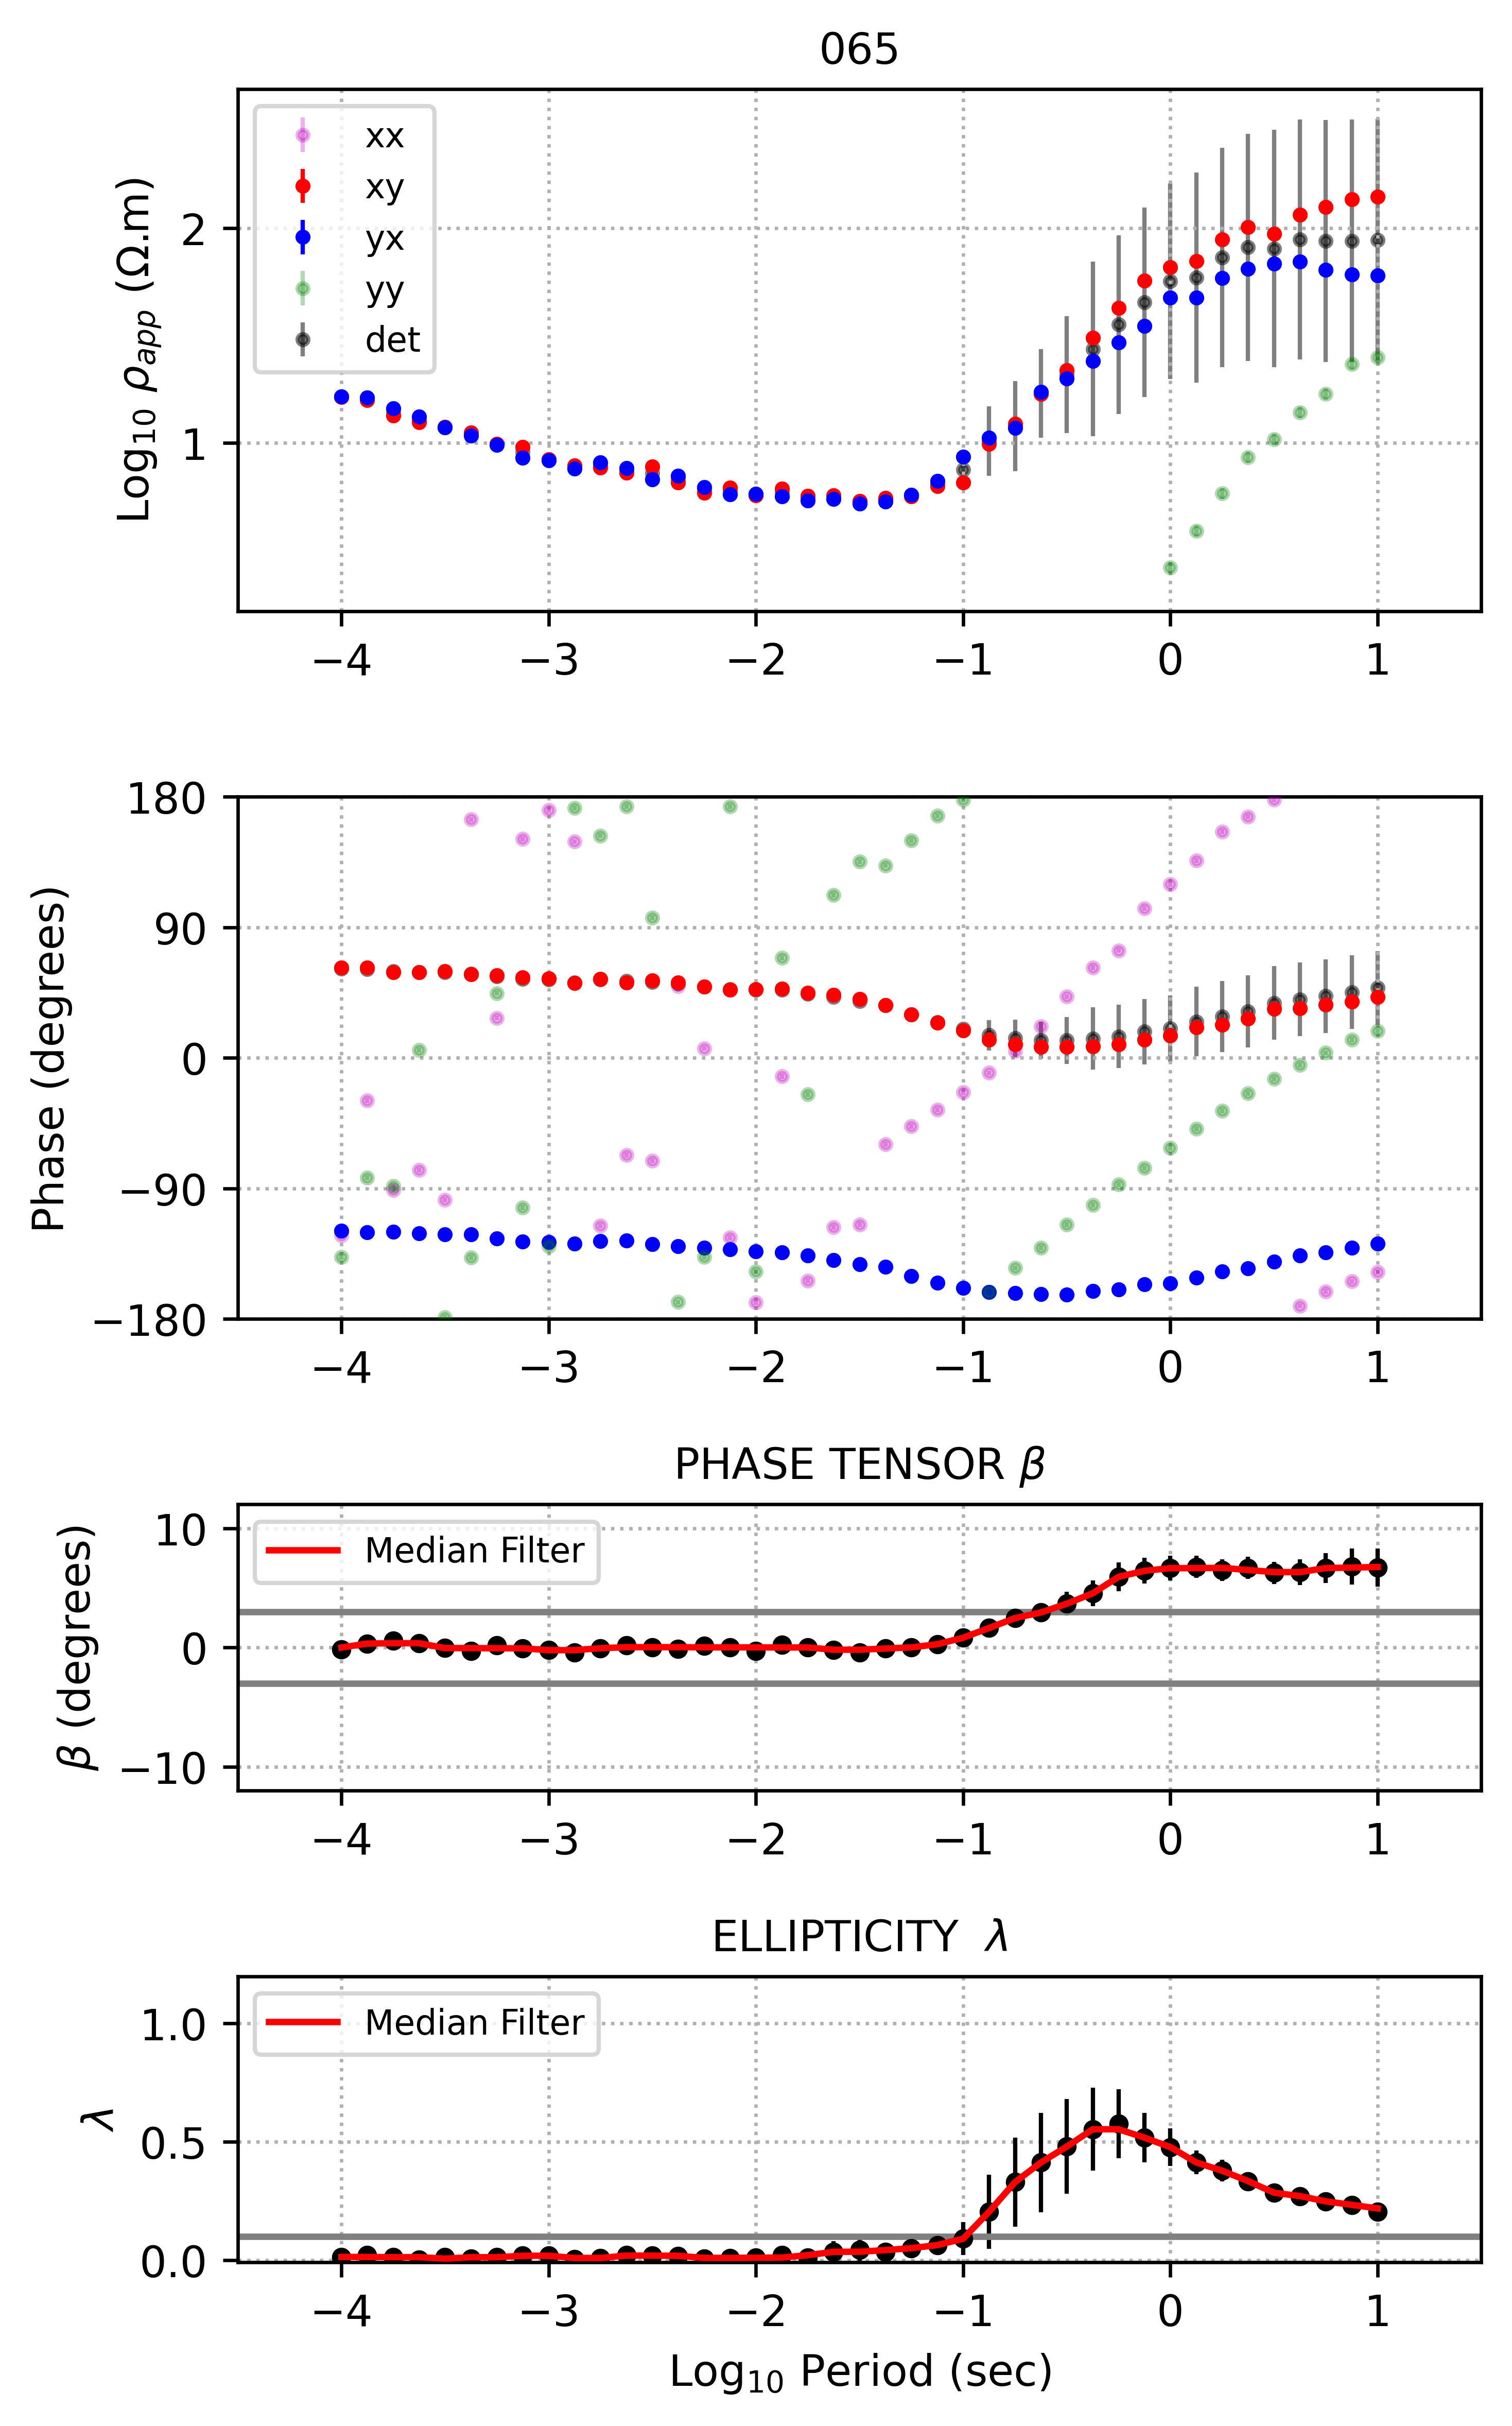
\includegraphics[width=0.33\linewidth]{figures/065.png}}%
		\subfloat[MT071]{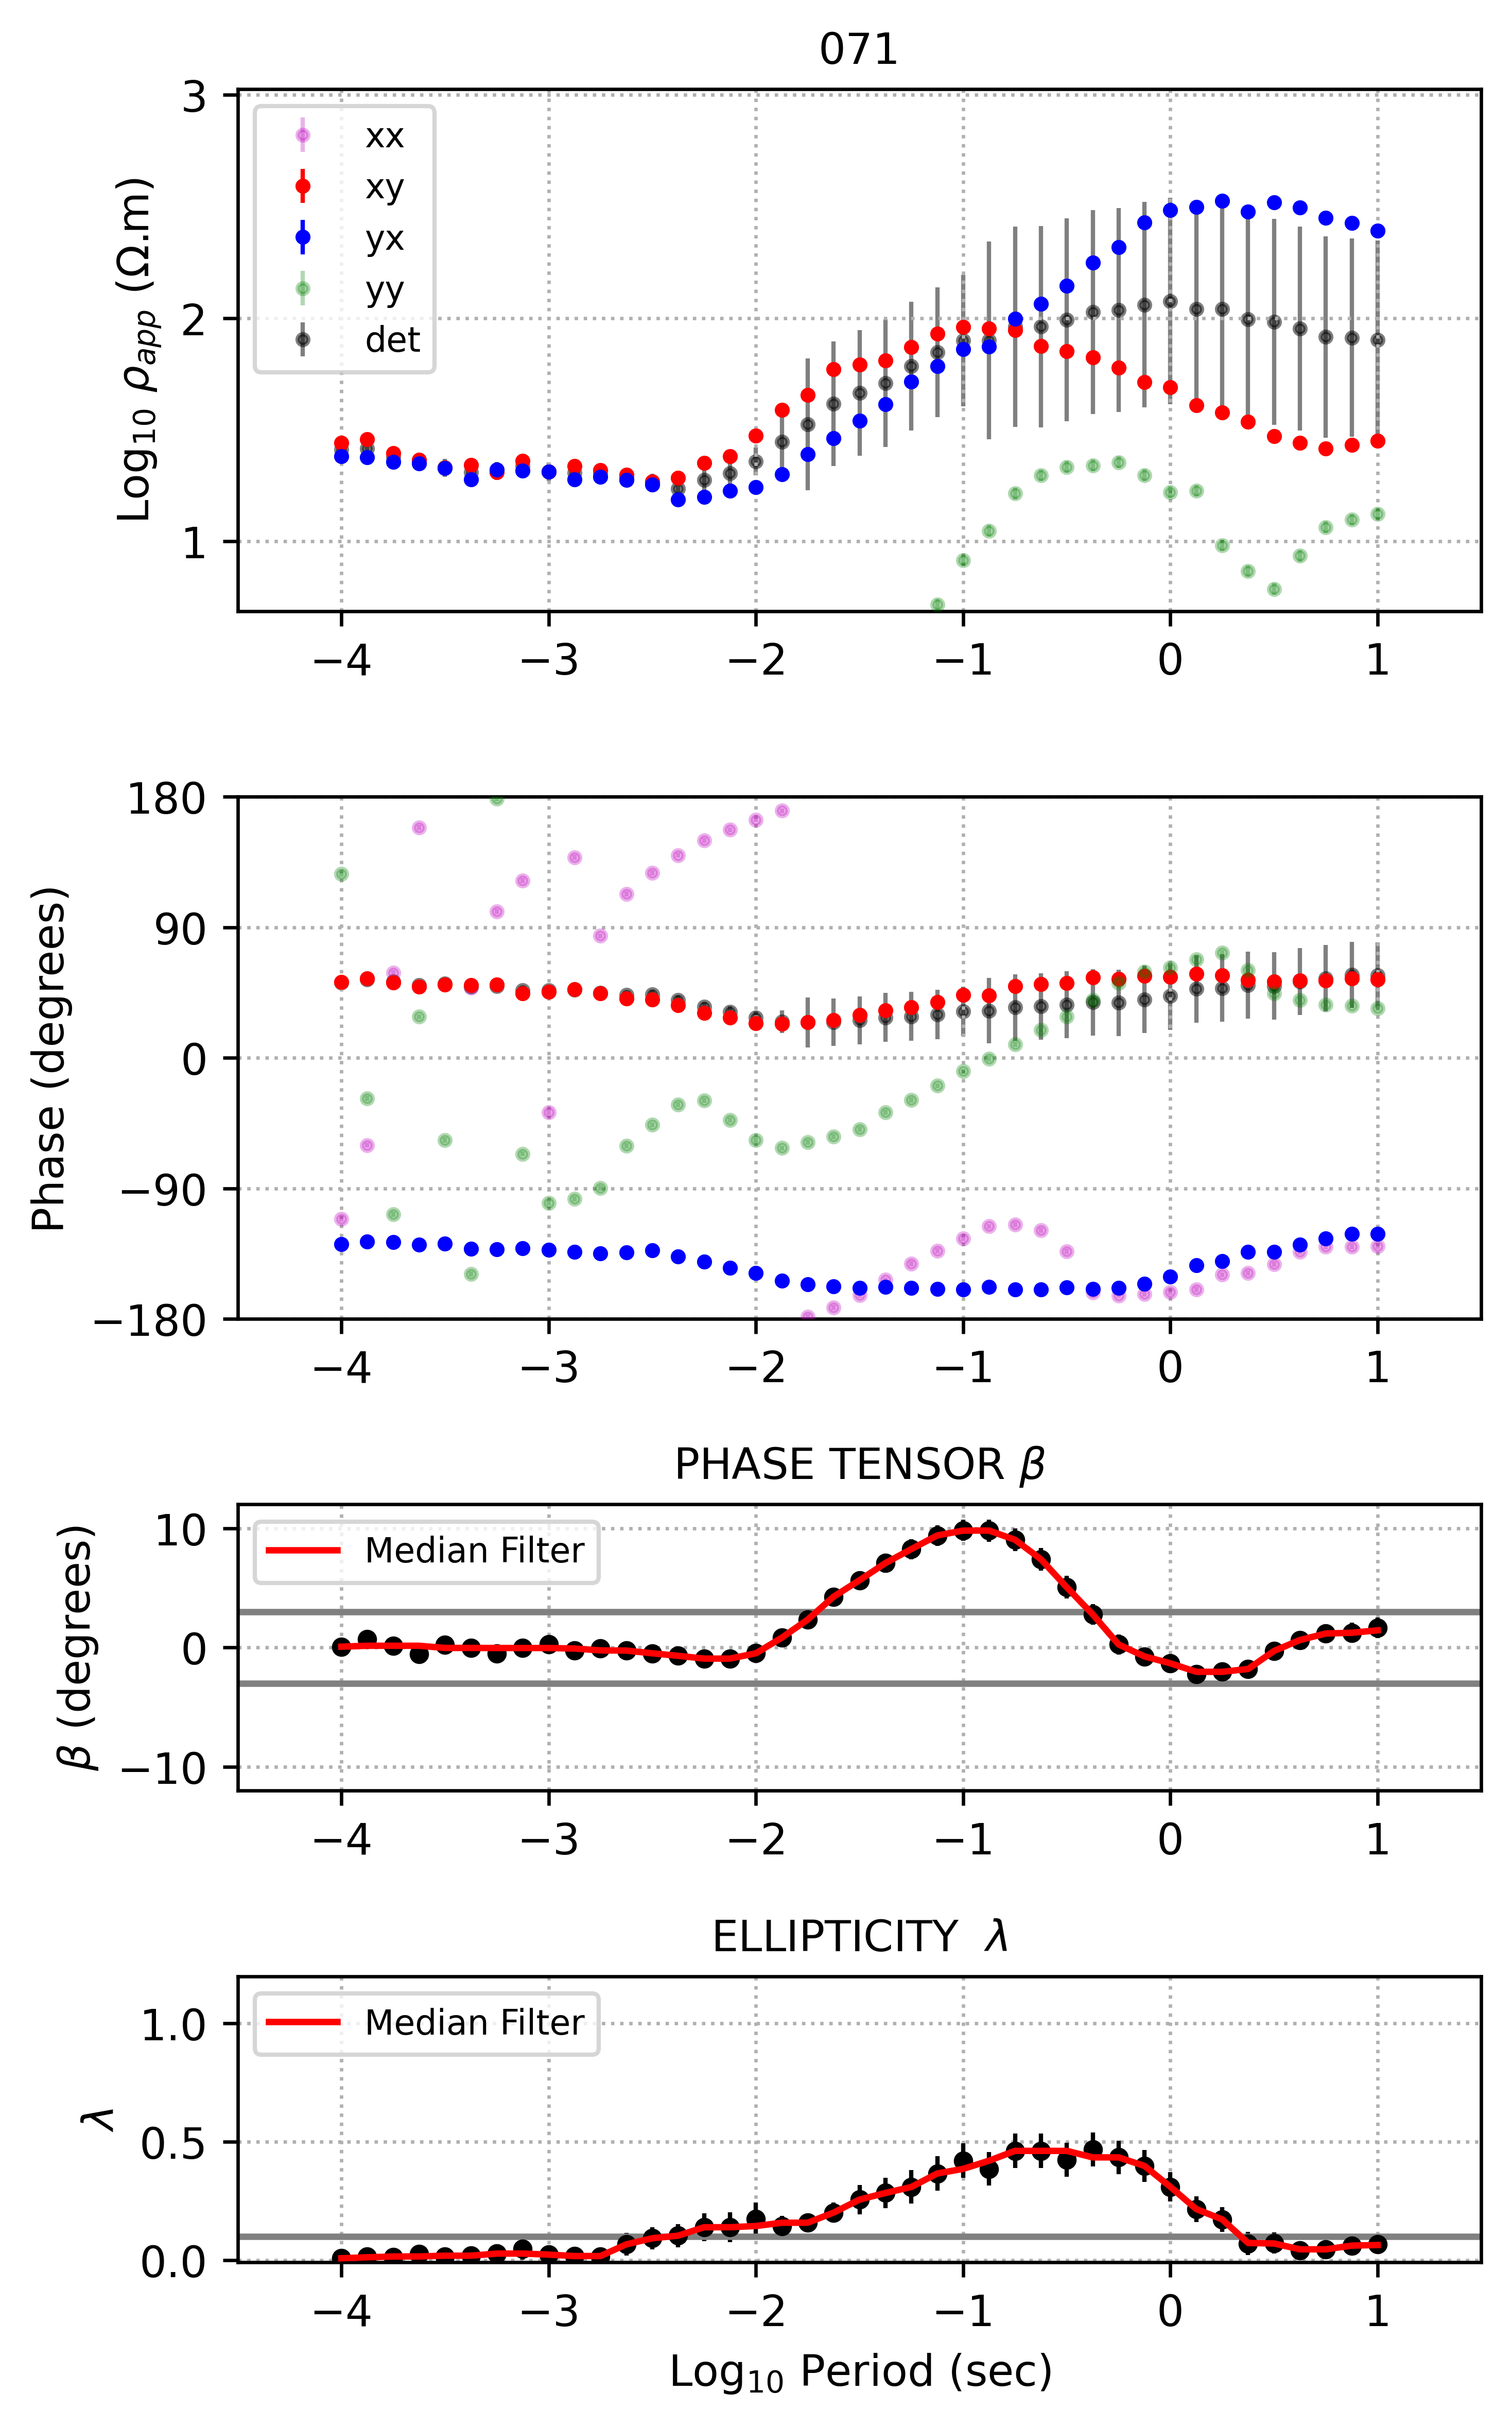
\includegraphics[width=0.33\linewidth]{figures/071.png}}%
		\subfloat[MT078]{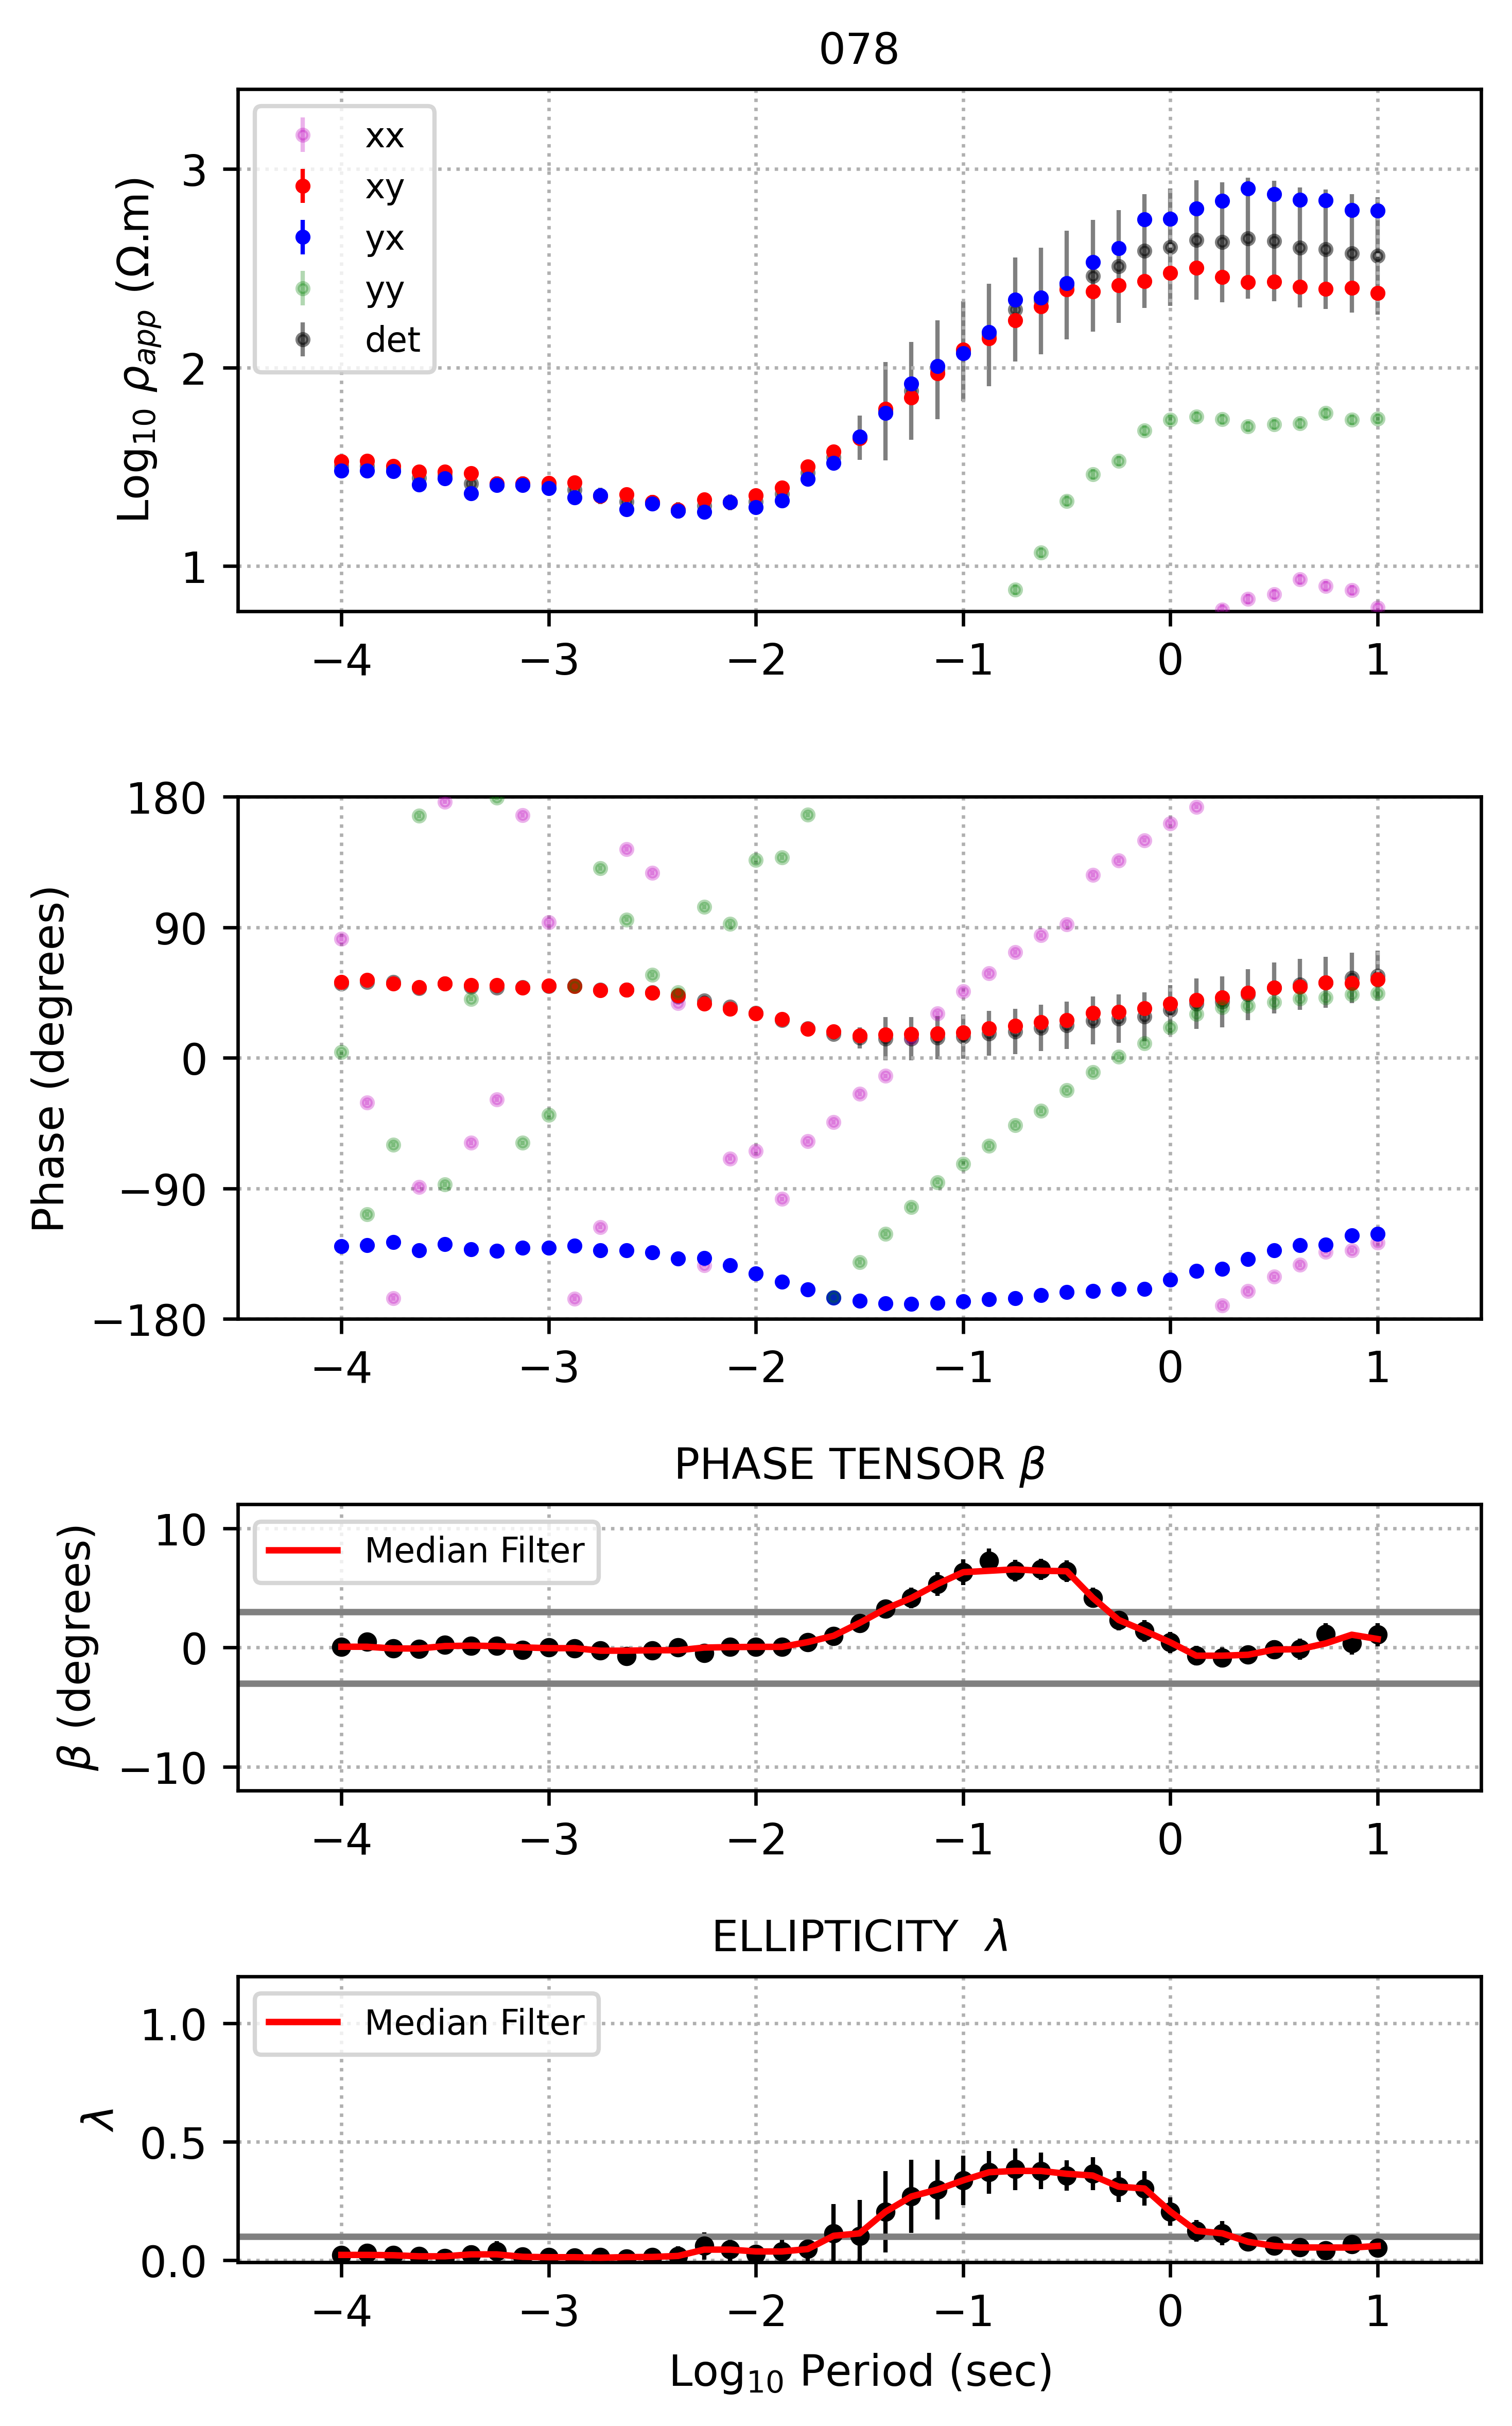
\includegraphics[width=0.33\linewidth]{figures/078.png}}%
		\caption{Plots created by the DDE.py script}
		\label{EDI2MTUL_figs}
	\end{figure}


	
	
	
	
	
	
	
    \section{transdMT} 	
    
    The \textbf{transdMT5} executable takes as input the .csv file and outputs an ensemble of models  that fits the data within its estimated uncertainty. 
    
     	Usage of the executable:
     	
    \begin{verbatim}
    main gamma ipfile runc infile outpath [-s seed] [-p samples] 
    [-h min max mean std] [-u min max] [-t startT]
    \end{verbatim} 

	For example, from \textit{projects/example/}:
	\begin{verbatim}
	../../src/transdMT5 2 ./transdMT/ipfile.csv 200000 
	  ./csv/065.csv ./transdMT/outfolder -s 100 -u -2 6
	\end{verbatim} 

    This command will run 1 Markov chain with 200.000 iterations for site 065, using an uniform resistivity prior between -2 and 6 log10 ohm.m, and a depth dependent prior as specified in ipfile.csv. The results (ensemble of responses and models) will be found in the outfolder. Running a single chain can provide a quick way to check the inversion/data is working properly. 
    
    Alternatively a \textit{parameters.txt} containing the inversion parameters can be used.    
	The \textit{parameters.txt} file allows to specify the parameters to use within the inversion using this format:
	
	\begin{verbatim}
	nChainsPar=4      --> number of chains to run in parallel
	nChainsTot=20     --> total number of chains 
	runc=1000000      --> number of mcmc iterations per chain (int >= 1000)
	ipfile=ipfile.csv --> depth dependent prior file 
	gamma=2           --> 1 for random layer widths, 2 for more equal layer widths
	samples=100       --> number of models to record (int>=1, default = 200))
	prior='-u'        --> use '-u' for uniform log10(res) prior
	                  --> use '-h' for truncated gaussian log10(res) prior
	min=-2    --> minimum of log10(res) (double, default = -3))(for uniform prior only)
	max=6     --> maximum of log10(res) (double, default = 6))(for uniform prior only)
	#mean=2   --> mean of log10(res) (double, default = 2))(for gaussian prior only)
	#std=  4  --> std dev of log10(res) (double, default = 4))(for gaussian prior only)
    \end{verbatim} 
    
	This example is run using an uniform prior on the resistivity, 20 chains are run, 4 at a time in parallel, with 1.000.000 iterations in each chain.   
    We recommend to run a minimum of 60 chains for 1.000.000 iterations each chain. Computing time will depend on the number of frequencies (i.e. data points) the MT sounding contains.
	% a word on the convergance of the different chains


	\bigbreak
	To run in batch several inversions, with several chains running in parallel, in  the \textit{project/example/transdMT} folder in a terminal run this command:
	\begin{verbatim}
	./batch.sh parameters.txt 
	\end{verbatim} 

	The inversion will be performed for all the .csv files located in the \textit{projects/example/csv/} folder. 	
	The ensemble of models \textit{sampModels} and responses \textit{sampResps} for each site, along with the input csv files will be generated in the \textit{project/example/trandMT/outfolder}.	
	
	
	\subsection{Depth dependent prior file}
	
	The depth dependent prior file defines the prior information on the expected number of layers within certain depth intervals. Using this prior allows to encourage complexity within certain intervals, but also discourage the apparition of unnecessary layers in intervals that are not constrained by the data. It is defined as follow:
	
	\begin{verbatim}
	division,rate
	5,1
	3000,5.5
	10000,2
	100000,2
	\end{verbatim} 

    The \textit{division} column defines the depth of the bottom of an interval. The \textit{rate} column defines the number of layers within that interval. If a uniform prior wants to be used, the file has to contain only one line, with the depth of the bottom of the model and the prior number of layers for the entire model. 
	
	
	
	
	
	
	
    \section{plotPosteriors} 	
	The script \textbf{plotResultsMCMC.py} plots the posterior distributions for the models and the responses. 
	\bigbreak
	\textbf{plotResultsMCMC.py}: Within the \textit{project/example/trandMT/} folder, run the script with these instructions:
	\begin{verbatim}	
	python3 plotResultsMCMC.py DepthMin DepthMax
	boolean_for_PLOT_PDF_RESPONSES boolean_for_plot_niblettBostick
	\end{verbatim} 
	For example:
	\begin{verbatim}
	python3 ../../../src/plotResultsMCMC.py 0 1500 True True
	\end{verbatim}
	
	Images created by the script for the EDI present in the example folder are shown in Fig. \ref{posterior_models} and Fig. \ref{posterior_fits}.
	
	
	\begin{figure}
		\centering
		\subfloat[Site-Specific Likelihoof Fcts]{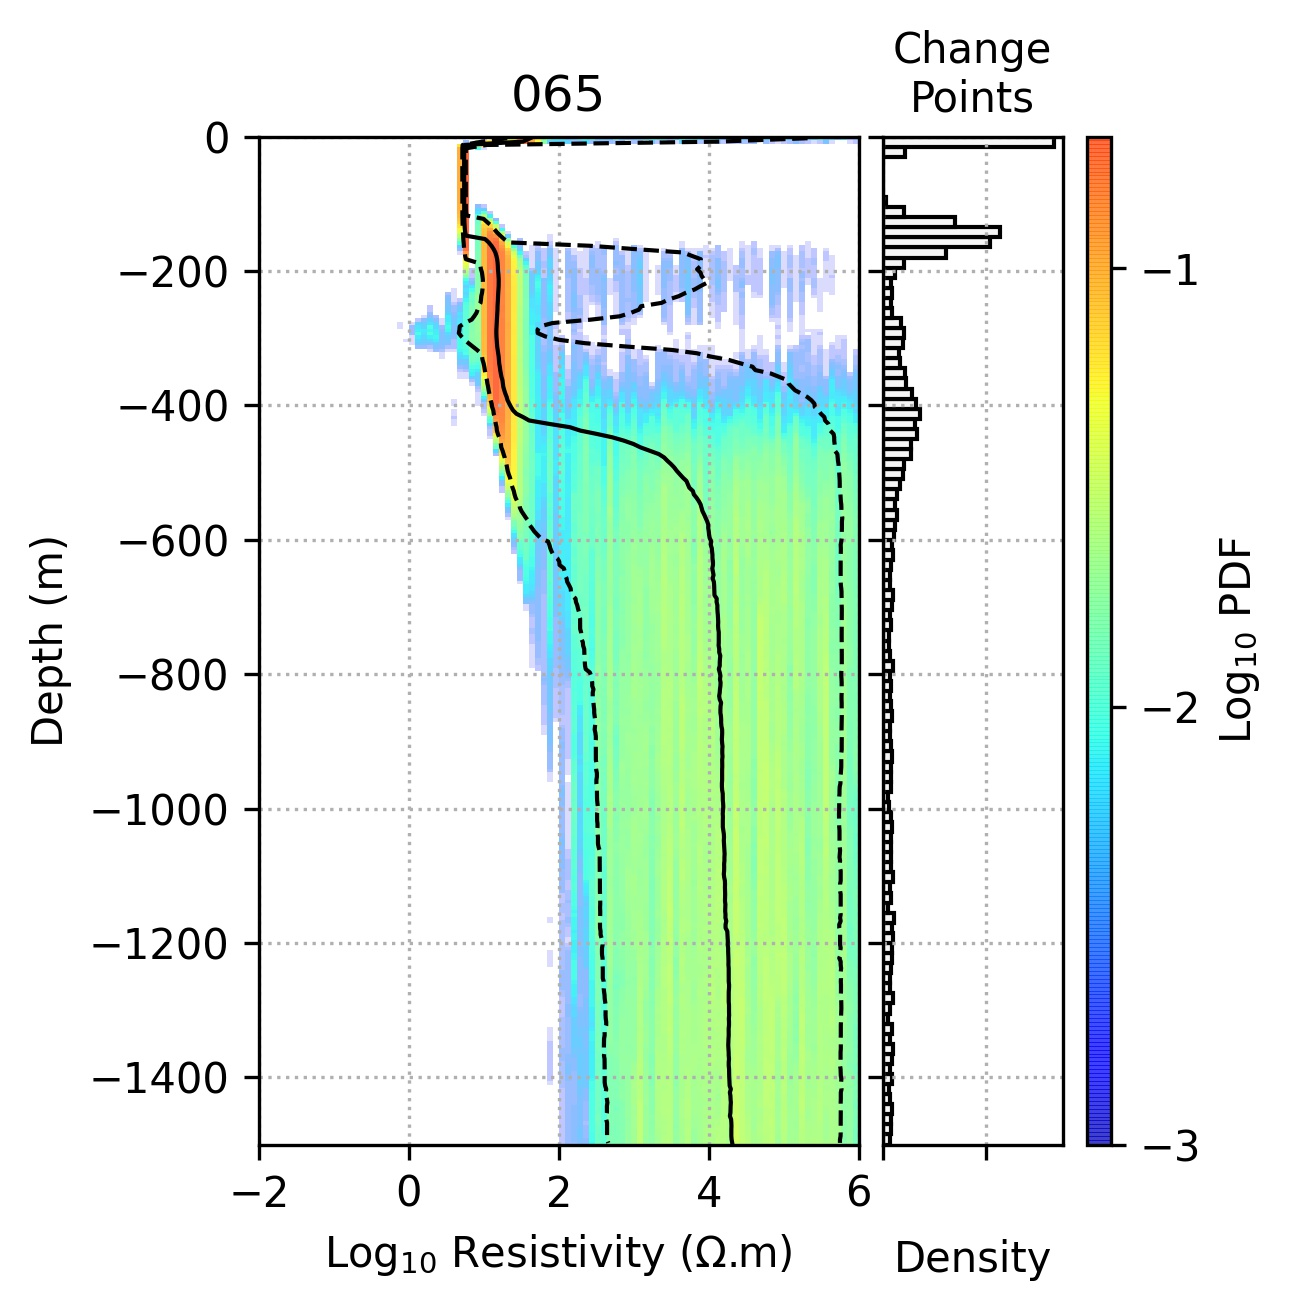
\includegraphics[width=0.5\linewidth]{figures/065_model.jpg}}%
		\subfloat[Error Floor 5\%]{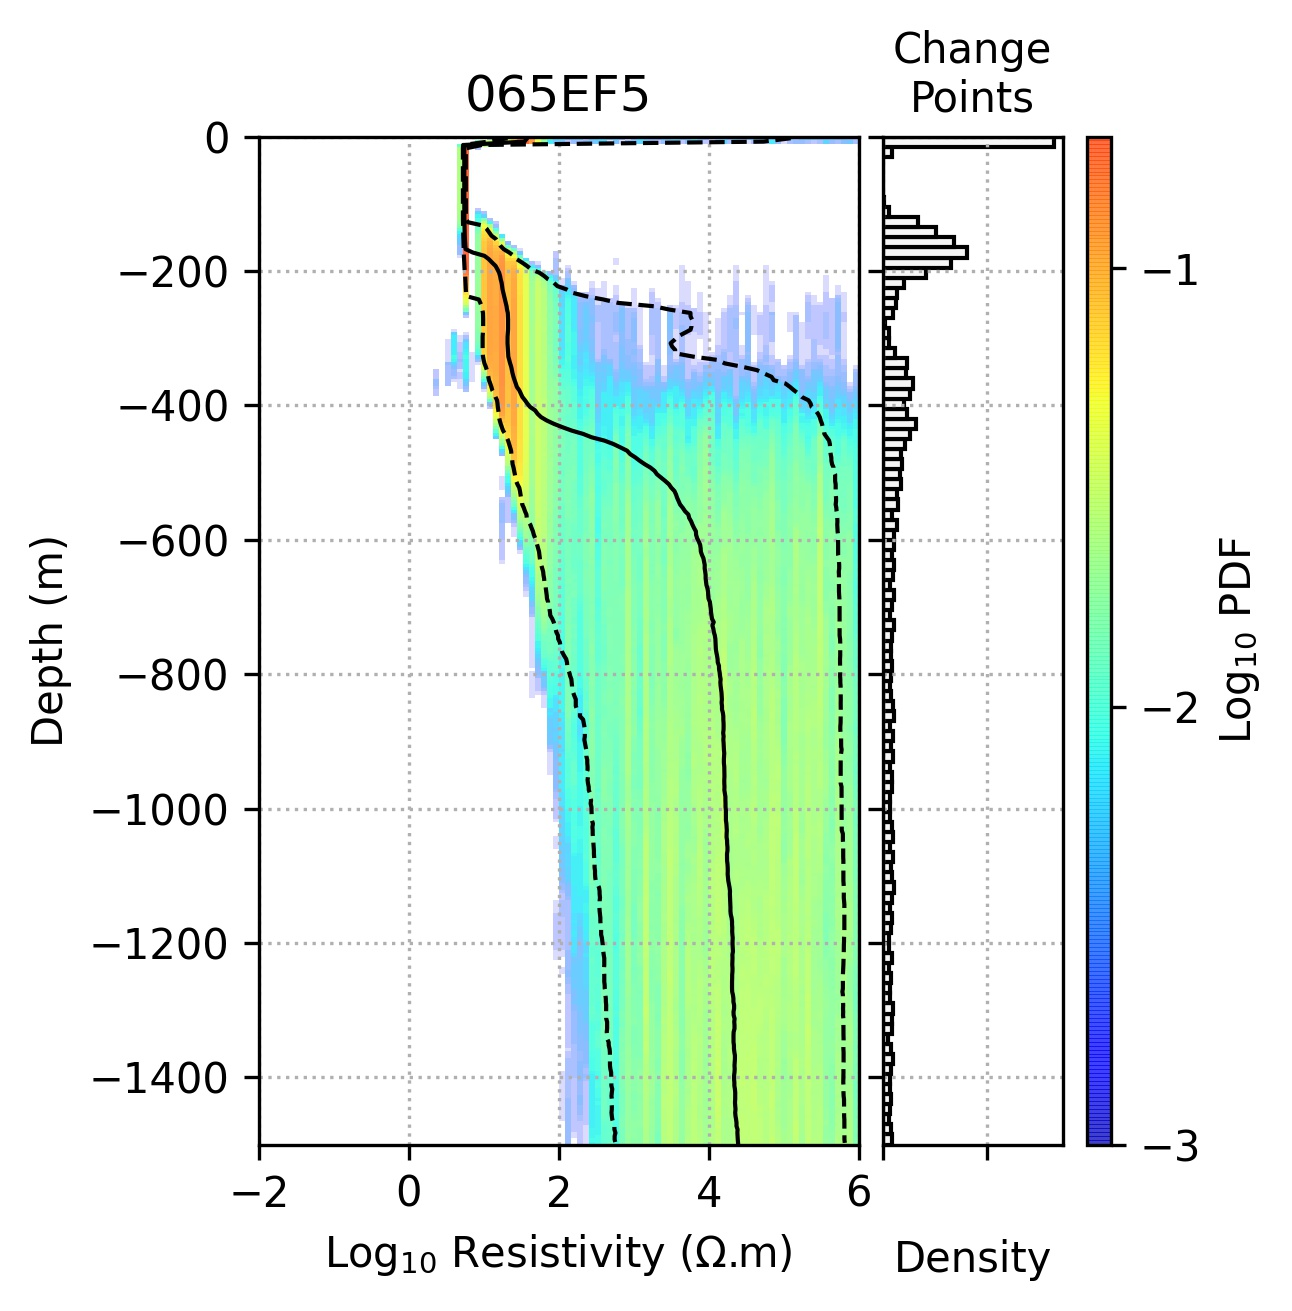
\includegraphics[width=0.5\linewidth]{figures/065EF5_model.jpg}}%
		\caption{Plots created by the \textit{plotResultsMCMC.py} script: Models posteriors.}
		\label{posterior_models}
	\end{figure}
	
	\begin{figure}
		\centering
		\subfloat[Site-Specific Likelihood Functions]{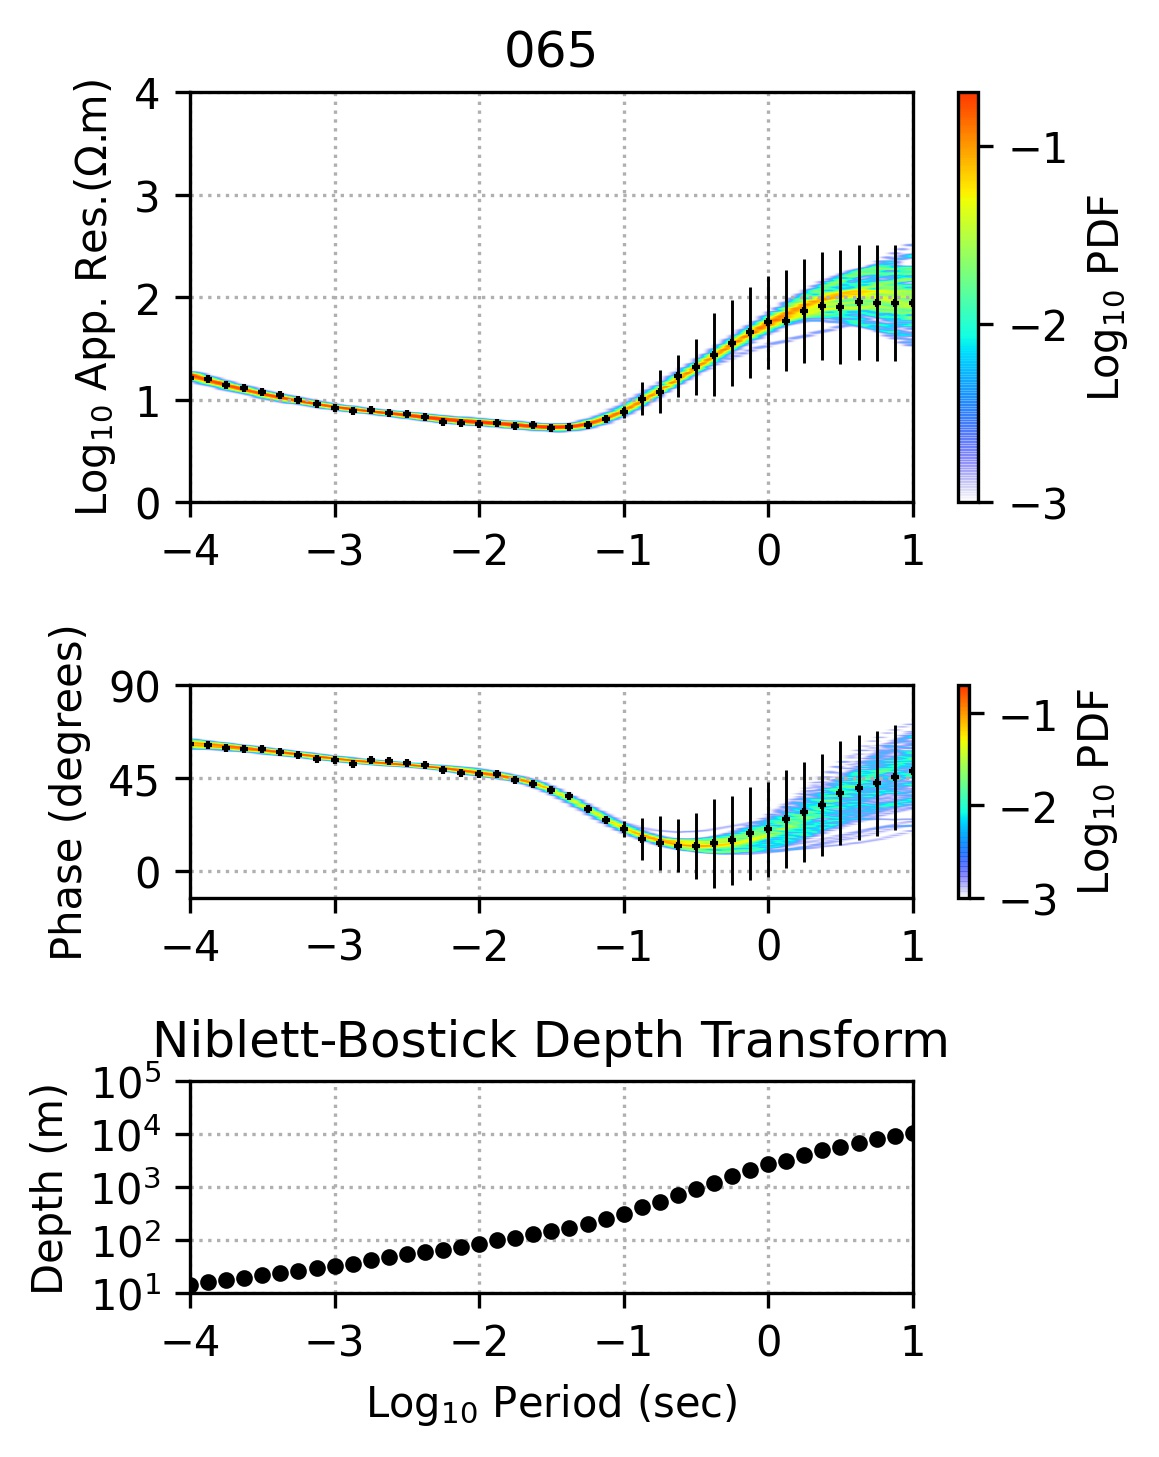
\includegraphics[width=0.5\linewidth]{figures/065_fit.jpg}}%
		\subfloat[Error Floor 5\%]{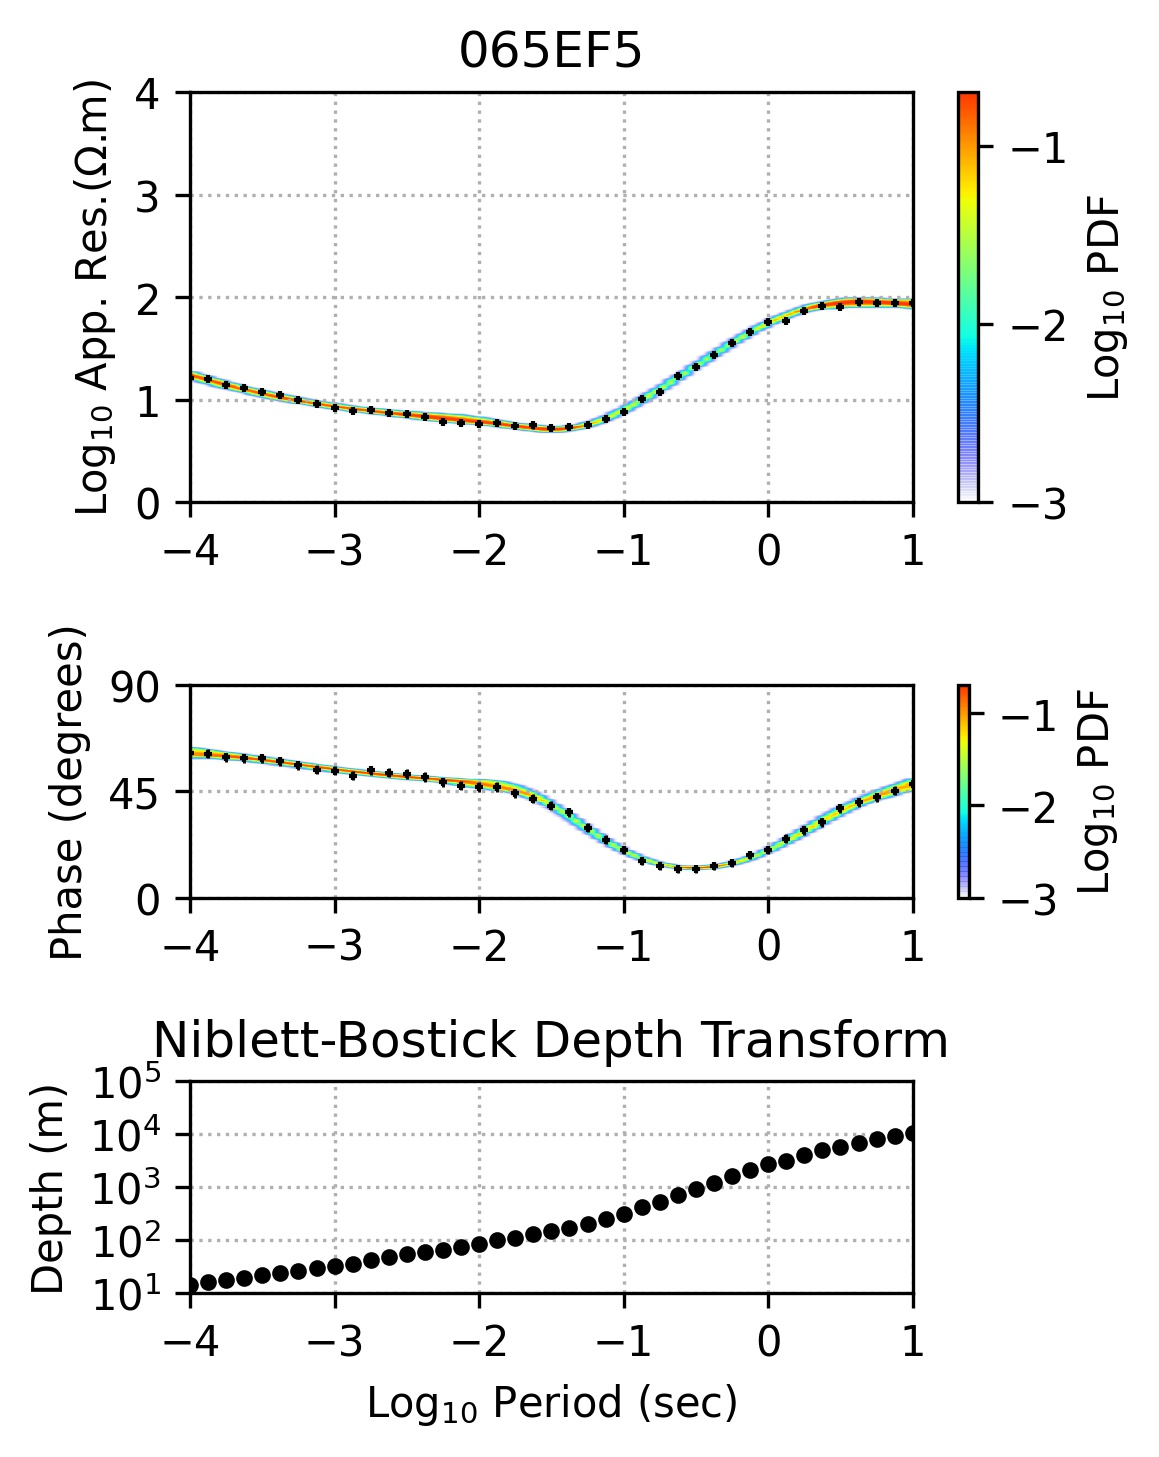
\includegraphics[width=0.5\linewidth]{figures/065EF5_fit.jpg}}%
		\caption{Plots created by the \textit{plotResultsMCMC.py} script: Responses posteriors.}
		\label{posterior_fits}
	\end{figure}
	\bigbreak	
	Option to plot the approximate Niblett-Bostick depth-transform is available.



    \section{Custom Tree} \label{custom_tree}
    
    This section describes the attributes file format and the tree file format, and how a custom tree can be constructed.
    
    \subsection{Attribute files}
    
    The attributes txt.file is constructed as follow:
    3 columns, comma separated:
    \begin{verbatim}
    condition number, condition name, condition
    \end{verbatim}  
    
    Example:   
    \begin{verbatim}	
	1,'elip1',elip > 0.1
	2,'elip2',elip > 0.2
	3,'elip3',elip > 0.3
	...
	7,'beta1',abs(beta) > 1
	8,'beta2',abs(beta) > 2
	...
    \end{verbatim} 
    
    The condition numbers have to match the ones in the tree file.
    
    \subsection{Tree file}
    
    The tree file is constructed as follow: 
    
    1st line: variogram
    
    2nd line: variogram
    
    from 3rd line to the end: 3 columns, white space separated
    
    \begin{verbatim}
    tree root number, tree node characteristic (split or leaf), 
           std dev (if leaf) or condition number (if split)
    \end{verbatim}  
    
    Example:   
    \begin{verbatim}
    1.8999999999999997
    0.7983039513625659
    0 Split 2
    1 Split 8
    2 Split 5
    3 Split 9
    4 Leaf 0.575751 
    4 Leaf 0.537254 
    ...    
    \end{verbatim} 
    

    The standard deviations (in log scale) for each data point is found at the leafs of the decision tree given the conditions established on the dimensionality attributes.
    
    The tree goes first to the "True" binary condition result.
    
    
    The variograms parameters define how the errors are correlated across adjacent frequencies. 
    
    
    \subsection{Construction of a simple tree}
    
    Here is how would look like a simplistic tree defined using 2 attributes:
    \bigbreak
    
    \textbf{Attributes file}
    
    \begin{verbatim}
	1,'elip1',elip > 0.1
	2,'beta1',abs(beta) > 3
    \end{verbatim} 


    \textbf{Tree file}

	\begin{verbatim}
	2               
	1
	0 Split 1
	1 Split 2     --> if elip > 0.1    
	2 Leaf 0.6    --> if abs(beta) > 3 (3D)
	2 Leaf 0.2    --> if abs(beta) < 3 (2D)
	1 Split 2     --> if elip < 0.1
	2 Leaf 0.6    --> if abs(beta) > 3 (3D)
	2 Leaf 0.03   --> if abs(beta) < 3 (1D)
	\end{verbatim} 
	
	
	Note that the standard deviation defined here and the variogram parameters set here are arbitrary. 



    \section{Notes}
    
    While the algorithm is designed to include either a DDM or to use error floors, it will be possible in a future version to include both simultaneously: when the Earth is relatively assimilable as uni-dimensional, the errors (processing + DDM) might still remain very low. This could be incompatible with the user's understanding of other sources of uncertainty (underestimated processing errors, physical assumptions). Then, this could be accounted for incorporating them within an error floor, used simultaneously with the DDM. 
    
    In a future version we will also add the possibility to invert for different components of the impedance tensor (TE/TM) or the the sum of the squared impedance elements (SSQ-impedance) \citep[see][]{Rung-Arunwan2016}.

	\bibliographystyle{apa}
	\bibliography{ref}

	\end{document}